\documentclass[20pt,margin=1in,innermargin=-4.5in,blockverticalspace=-0.25in]{tikzposter}
\geometry{paperwidth=42in,paperheight=32.5in}
\usepackage[utf8]{inputenc}
\usepackage{amsmath}
\usepackage{amsfonts}
\usepackage{amsthm}
\usepackage{amssymb}
\usepackage{mathrsfs}
\usepackage{graphicx}
\usepackage{adjustbox}
\usepackage{enumitem}
\usepackage[backend=biber,style=numeric]{biblatex}
\usepackage{uwtheme}

\usepackage{mwe} % for placeholder images

\addbibresource{refs.bib}

% set theme parameters
\tikzposterlatexaffectionproofoff
\usetheme{UWTheme}
\usecolorstyle{UWStyle}

\usepackage[scaled]{helvet}
\renewcommand\familydefault{\sfdefault} 
\usepackage[T1]{fontenc}


\title{ETERNITY: NUMBERS - PI}
\author{Baiyu Huo \textsuperscript{$\dagger$}}
\institute{\textsuperscript{$\dagger$} SOEN 6481 - Software System Requirements Specification }
\titlegraphic{
\includegraphics[width=0.18\textwidth]{assets/logo.jpg}}

% begin document
\begin{document}
\maketitle
\centering
\begin{columns}
    \column{0.32}
    \block{Introduction}{
         The project is about making a calculator which computes the eternity number PI from scratch and provides some related applications which related to PI. The whole project contains the following phrases:
          \begin{itemize}
     \item  Understanding the problem domain.
     \item  Collecting the requirements by performing an interview with expertise.
     \item  Documented the requirements (use case, UML diagram, maintain the requirement traceability ).
     \item  Implementation.
    \end{itemize}
    
    The primary task in this project is about the PI and its functions. PI is a mathematical constant which people has been doing research on for a long time and being applied in a lot of famous mathematical problem solutions. In this project, the PI was calculated in 2 different algorithms and 6 different degrees of precision. Besides the general functions in the calculator, The calculator provides "calculate the area of a circle" and "calculate the circumference of a circle" --- two extra functions that need to use the PI. 
        \begin{tikzfigure}[PI (Source: Google)]
            
\includegraphics[width=0.4\linewidth]{assets/PI.jpg}
        \end{tikzfigure}
    }
    \block{Critical Decisions}{
    \section{ The Selection of Interviewee }
        Because PI appears in many formulas in all areas of mathematics and physics, the choices of the interviewee in this project have to narrow down to the people who have mathematics and physics background or work in related fields.  
        
      Dr. Wang and Ms. Xuan are two candidates for the interview. Dr. Wang is a mathematical course lecturer in college, Ms. Xuan, on the other hand, works as a bank accounting with a bachelor in mathematics degree. At this stage, the character of the candidates became a very important factor. Finally, Dr. Wang was chosen due to the his spontaneous nature which eased the flow of the interview.

    \section{ Decisions about the functions }
  Besides the general functions in the calculator, there are a lot of applications which use PI in the user story such as  "circle area calculation", "circle circumference calculation" and " Trigonometry calculation".  According to the time limitation, only one or two of them can be implemented. The final decision was made in terms of the degree of relation and, implementing efforts and the feedback from the interviewee which also be considered as the customer of the project. For implementing the trigonometry calculation, the function of sin, cosine and tan need to be implemented, which was hard to finish within the project period, so the area calculation and circumference had been chosen.

    }
     \column{0.36}
       \block{Critical Decisions }{

  
    \section{ The Choice Between Precision or Performance  }
        Computing the PI is one of most important functions in this project.However, the more accurate pi being calculated, the more time it needs, which leads to low performance. But, both accuracy and performance are important in a different scenario.  After analyzing each of the scenarios, the final decision is to give an extra function to users  to choose the degree of precision of pi, so that they can tackle the problem in different situations.
              \begin{tikzfigure}[Decision among qualities (Source: Google)]
            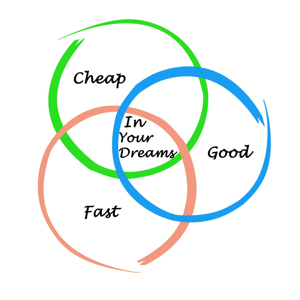
\includegraphics[width=0.4\linewidth]{assets/fast-cheap-good.png}
        \end{tikzfigure}
        
    \section{ Trade offs for architecture }
    
 The project was designed to have multiple qualities such as high extensibility, high maintainability, which requires the component to achieve modularity, high cohesion and low coupling. To achieve those features, a set of design patterns are applied in this project, such as singleton pattern, memento pattern and strategy pattern. It increased the extensibility of the program and increased the understandability for the maintainer. However, applied too many unnecessary patterns is also not a good thing, so there are some trade-offs about the architecture of the project. The pattern would only be applied when certain qualified need to be achieved. What's more, the project is designed under the SOLID principles, especially the open-close principles. 
               \begin{tikzfigure}[SOLID (Source: Devopedia)]
            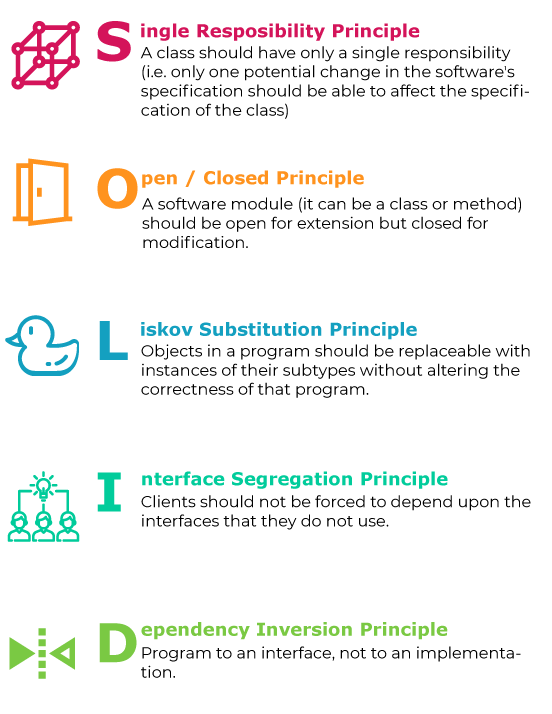
\includegraphics[width=0.5\linewidth]{assets/solid-principle.png}
        \end{tikzfigure}
       }
     \column{0.32}
    \block{Challenges}{
    \section{ Time Limitation }
     As the length of the project is only 3 weeks, it is a kind of challenge to understand the knowledge about requirement engineering and applied them in the project. Since the software is a process, as we mentioned at the beginning of the poster, there are 4 phases in the project which map the different phase of the software life circle except for the maintenance phases.
    
    \section{ Understand Mathematical problem domain }
     Because I don't have any background in mathematics, so the calculation of pi is one of the main challenges for me. After research, I got two algorithms from the internet, however, it is hard for me to understand the theory of it.  
         \begin{tikzfigure}[Math (Source: Youtube)]
            
\includegraphics[width=0.5\linewidth]{assets/maxresdefault.jpg}
        \end{tikzfigure}
     
    \section{ Implementation of math function in java }
    According to the instruction of the project, we can not able to used any build-in functions in java.math package, so we implement the functions such as Square root, power and PI.
    }
    
    

    
    \block{Lessons}{
    \begin{itemize}
     \item Embrace the challenges, even that means you need to jump out of your comfort zone.
     \item Never put off until tomorrow what you can do today.
     \item Communication is really important in software requirement.
     \item You need to understand the problem domain first, before making the decisions during the software engineering process.
    \end{itemize}
    }


    \block{References}{
        \begin{itemize}
     \item  [1] Wikipedia contributors. Pi — Wikipedia, the free encyclopedia, 2019. [Online; ac-cessed 6-Augest-2019].
     \item  [2] Wikipedia contributors. SOLID — Wikipedia, the free encyclopedia, 2019. [Online; ac-cessed 7-Augest-2019]
     \item [3] Projectsmart contributors. understanding-the-project-management-triple-constrain, 2019. [Online; ac-cessed 7-Augest-2019]
    \end{itemize}

    
   
    

    }
    
\end{columns}
\end{document}